%%%%%%%% symbols to add
\simbolo{f(x,y)}{Original image as a function of spatial coordinates $x$ and $y$}

\simbolo{g(x,y)}{Observed image as a function of spatial coordinates $x$ and $y$}

\simbolo{J_{1}}{Bessel function of the first kind}

% \simbolo{\eta}{Additive noise function}

% \simbolo{\ast}{Convolution operation}

% \simbolo{\delta}{Dirac delta function}

% \simbolo{\mathbb{R}}{Set of real numbers}

% \simbolo{\mathbb{N}}{Set of natural numbers}

% \simbolo{\wedge}{Diagonal matrix of decrescent multiple singular values}

% \simbolo{\mathbb{G} = (\mathbb{V},\mathbb{E})}{Graph}

% \simbolo{\mathbb{V}}{Set of vertices of a graph}


The human eye constructs images from incident light rays on the \emph{retina}, a very complex set of photoreceptors that converts light into electrical signals which are later interpreted by the brain. The result of this process may be modelled as continuous function of two variables $f(x,y)$ which comprises the \emph{illumination} and the \emph{reflectance} information, i.e. the amount of incident light and the amount of reflected light in the scene, respectively \cite{gonzalez2018digital}.

Digital image processing deals, as the name proposes, with \emph{digital images}, i.e. discrete representations of $f(x,y)$ generated by sensors that are capable of transforming the illumination and reflectance information into electric signals. Still according to \citeonline{gonzalez2018digital}, in order to achieve this representation, the signals undergo sampling (signal conversion from continuous to discrete) and quantization (mapping of real-valued intensities to discrete pixel values) processes. For the sake of notation simplicity, $f(x,y)$ denotes the digital image and the term ``image'' also refer to it along this work.

It is clear that the image formation is influenced by several factors: sensor type, scene illumination conditions, and others. Indeed, each imaging system such as a camera or a microscope adds its own constraints to the process, e.g. conventional transmitted light microscopy images are only achieved with non-opaque samples \cite{rudi2020contrast}. Although there are many types of microscopy with different imaging procedures, this work limits its scope to bright-field microscopy. Therefore, this chapter summarizes the bright-field microscopy image formation processes and its implications on quality of the images. Furthermore, it describes blur properties concerning its origins either in image formation or other events. 


\section{Image Formation}

As mentioned in chapter \ref{chapter:fundamentals-of-optics-and-light-microscopy}, the bright-field microscopy images are formed by either transmitted or reflected light that passes through the sample and reach the objective lens. There difference between transmitted light and reflected light microscopes is the illumination system; there is no difference in how both direct light rays after those leave the specimen \cite{leng2009materials}.

According to \citeonline{davidson2002optical}, the light which reaches the specimen is either undeviated, i.e. does not suffer any disturbances in its direction, or diffracted; the diffracted rays leave the sample with a phase difference of 180 degrees in comparison to the undeviated light and cause destructive interference in the eyepiece, which projects a magnified version of this pattern onto a sensor and consequently produces the image.

Furthermore, the diffraction patterns that are captured by objectives have a particular shape. Still as stated by \citeonline{davidson2002optical}, the \emph{Airy disks}(also called \emph{Airy patterns}), named after Sir George Biddell Airy (1801 - 1892), are small circular diffraction disks projected by the objectives onto the image plane of the eyepiece diaphragm, which describe the focus profile the resulting image. The Airy disks as described by \citeonline{fowles1989introduction} follow the Fraunhoffer diffraction pattern, and may be mathematically modelled as an angular distribution of intensity of light diffracted by a circular aperture, given by

\begin{align}
\label{eqn:airy_function}
I(\theta) = I_{0} 
            \left[ 
            \frac{2 J_{1} (\rho)}{\rho}
            \right]^{2}
&&
\rho = \left( 
        \frac{2 \pi \sin{\theta}}{\lambda}
        \right) \frac{a}{2},
\end{align}

\noindent where $I_{0} = (C \pi R^{2})^{2}$ is the intensity for $\theta = 0$, $C$ is a constant, $R$ is the radius of the aperture, $\lambda$ is the wavelength of the light, $a$ is the diameter of the aperture and $J_{1}$ is the Bessel function of the first kind and first order \cite{mathews1970mathematical}, where the general case for the $rth$ order is given by

\begin{align}
\label{eqn:1st_bessel}
J_{r}(x) = \sum_{n = 0}^{\infty}
            \frac{(-1)^{r}}
                 {r! \Gamma(m + r + 1)}
            \left(
                \frac{x}{2}
            \right)^{m + 2r}
&&
\Gamma(z) = \int_{0}^{\infty} e^{-u} u^{z-1}du
\end{align}

The Airy disks are intrinsically related to the numerical aperture and the definition of \emph{resolution}. The resolution is the minimum distance between two points at which they can be visibly distinguished as two points; optically, it is defined as the minimum distance between two Airy disks that can be distinguished, which is limited by diffraction \cite{leng2009materials}. The resolution of an optical microscope, given by the Rayleigh equation, is described by

\begin{equation}
\label{eqn:resolution}
d = 1.22 \frac{\lambda}{2 NA},
\end{equation}

\noindent where $d$ is the space between two adjacent particles that may be distinguished from each other, $\lambda$ is the wavelength of the illumination and $NA$ is the numerical aperture of the objective \cite{davidson2002optical}. It is evident that objectives with higher numerical apertures and shorter wavelengths of visible light will yield better resolution. The Figure \ref{fig:airy_disks} shows arbitrary examples of Airy patterns, as well as their possible configurations and their consequences to the image. In Figure \ref{fig:airy_disks}.(a), the usual shape of Airy patterns is shown, together with its two-dimensional representation as a function of the intensity by an interval. Next, Figure \ref{fig:airy_disks}.(b) depicts an occurrence of Airy disk overlapping where both points would be properly resolved, i.e. below the Rayleigh limit, and Figure \ref{fig:airy_disks}.(c) represents the minimum distance in which both points would be distinguished. Finally, Figure \ref{fig:airy_disks}.(d) represents an unresolved pair of points.

\begin{figure}[htb]
	\centering
	\caption{\label{fig:airy_disks} Arbitrary example of an Airy disk (a), resolved Airy disks (b), Rayleigh limit of resolution (c) and unresolved Airy disks (d).} 
	\begin{center}
	    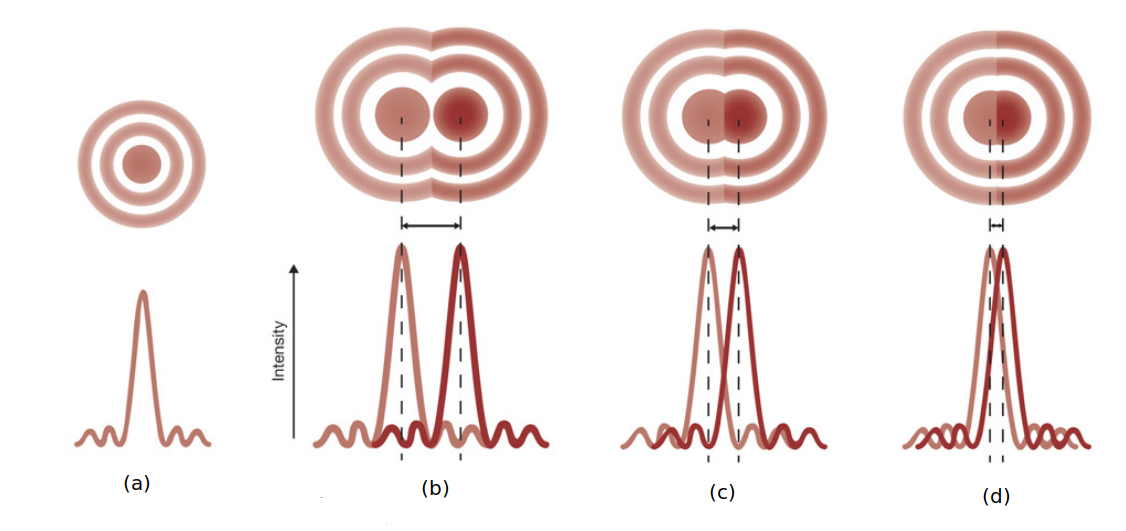
\includegraphics[scale=0.4]{images/airy_disks.png}
	\end{center}
	\centering
    \fadaptada{dunst2019imaging}
\end{figure}

As explained by \citeonline{goodman1996introduction}, an imaging system, particularly a set of microscope lenses, is said to be \emph{diffraction-limited} if the incident spherical light wave generated from a point-source object is transformed into another spherical wave which converges to an ideal image point, described by the original object point and affected by some sort of isotropic effect, such as magnification in a microscope.

The depth of field was described in chapter \ref{chapter:fundamentals-of-optics-and-light-microscopy} in terms of focal plane distances, but it may also be taken as the \emph{axial resolving power}, a measurement of resolution along the $z$ axis, determined by the numerical aperture and described by the Airy disk profile \cite{davidson2002optical}. Similarly to the Rayleigh's equation, the depth of field increases
with higher numerical apertures for the objective and shorter wavelengths of the incident light, and it represents a key property concerning the amount of blur in the resulting image.


\subsection{Point Spread Function and Image Formation Model}

\label{sec:point_spread_function_and_image_formation_model}

When light waves from a point source reach lenses, they suffer diffraction and refraction, which construct a new propagating set of rays that converge to a point in the center of the image plane in the shape of Airy disks; such shape is called the \sigla{PSF}{Point Spread Function}
of the imaging system (also called \emph{impulse response}), and it is intrinsically related to the imaging process \cite{wu2008microscope}. Particularly, the bright-field microscopy employs polychromatic nonpolarized incoherent light. From this concept, it is possible to relate the Airy disks to the PSF, since those are intensity distributions for each point source of light emanating from the specimen. Figure \ref{fig:point_spread_function}.(a) presents a theoretical scheme of imaging for a point source of light, and Figure \ref{fig:point_spread_function}.(b) depicts the shape of a incoherent PSF:

\begin{figure}[htb]
	\centering
	\caption{\label{fig:point_spread_function} Point Spread Function generated by a focused diffraction-limited system with incoherent light.} 
	\begin{center}
	    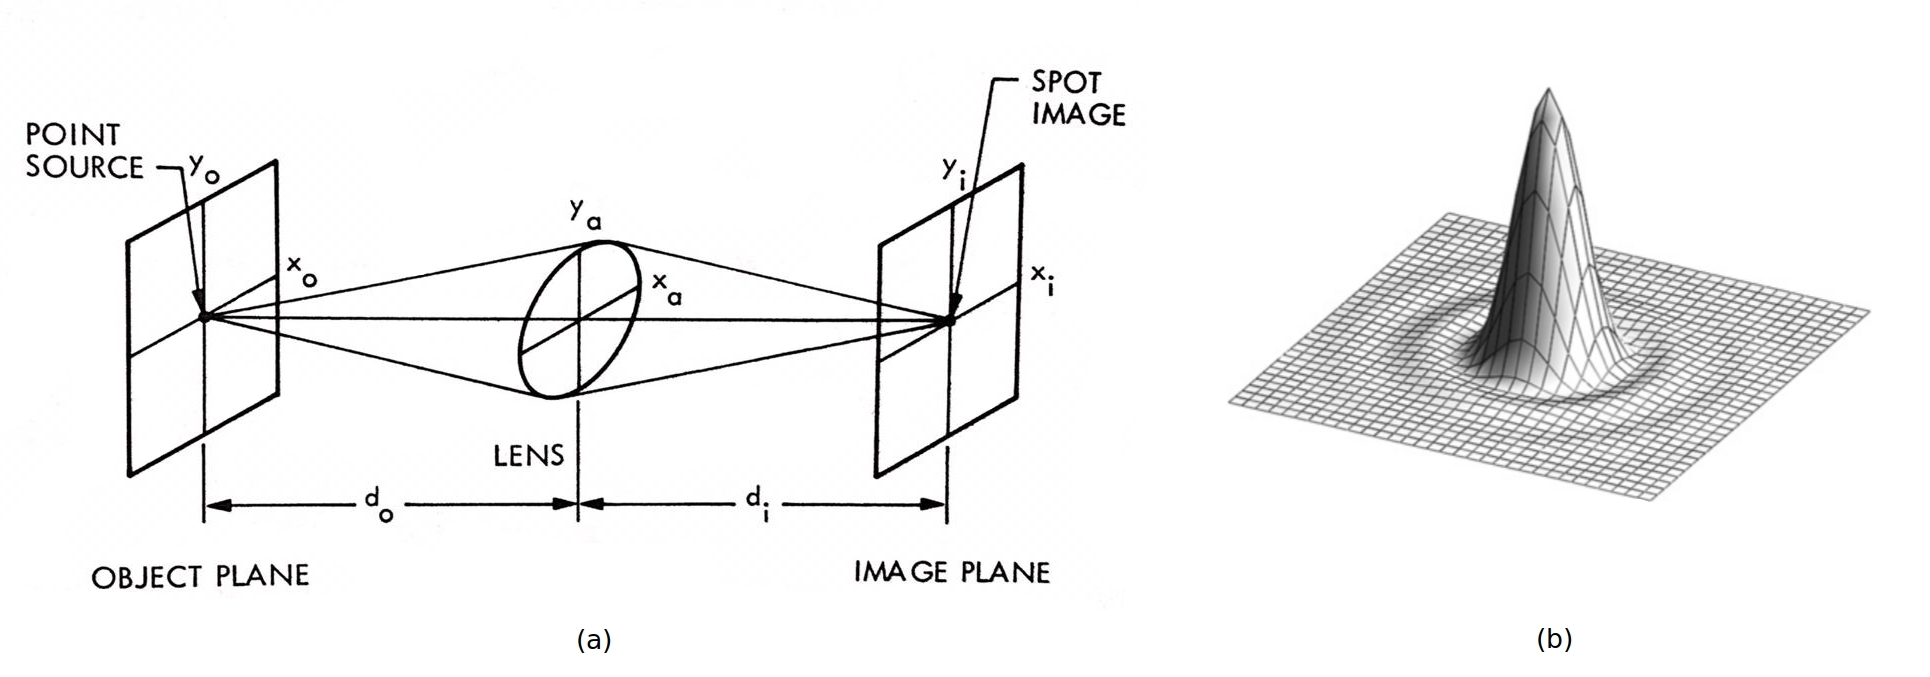
\includegraphics[scale=0.235]{images/point_spread_function.jpeg}
	\end{center}
	\centering
    \fadaptada{castleman1996digital,wu2008microscope}
\end{figure}

In Figure \ref{fig:point_spread_function}.(a), the imaging system in in focus, which is given by

\begin{equation}
\label{eqn:lens_focus}
\frac{1}{d_{o}} + \frac{1}{d_{i}} = \frac{1}{f},
\end{equation}

\noindent where $f$ is the focal length of the lens, $d_{o}$ and $d_{i}$ are respectively the distances from the point source plane to the lens and the distance from the image plane to the lens; the intensity of light in the point source is directly proportional to the intensity in the image, what characterizes a \emph{two-dimensional linear system} \cite{castleman1996digital}. Still according to \citeonline{castleman1996digital}, any motion of the point source on its plane moves the image is dictated by the law

\begin{align}
\label{eqn:isoplanatic_motion}
x_{i} = -\frac{d_{i}}{d_{o}}x_{o}
&&
y_{i} = -\frac{d_{i}}{d_{o}}y_{o},
\end{align}

\noindent where $(x_{o},y_{o})$ are the coordinates for the object location on its plane and $(x_{i},y_{i})$ are coordinates that locate the image on its plane. This implies that the shape of the image will not change according to the object's location, and this property yield \emph{shift invariance} to the system, which may be called \emph{isoplanatic}. These properties are observed in an ideal imaging system - simple lenses are not isoplanatic and linear, and  consequently simple microscopes also. However, there are approximations and mathematical tools that allow advanced microscopes to be assumed isoplanatic and linear.

The PSF as related to the intensity distributions described by the Airy disks are limited to the area of the aperture. This means that the amount of light that reaches the image plane is truncated by the circular aperture, what is also true for the PSF. The truncation is mathematically represented by the \emph{pupil function}, which is zero outside the boundaries of the aperture and unity otherwise, and might include also information about wave aberrations of the lens \cite{goodman1996introduction}. As denoted by \citeonline{wu2008microscope} with some notation adjustments, the PSF of an incoherent illuminated circular aperture imaging system is the Fourier Transform (explained further in Chapter \ref{chapter:theoretical-background}) of the generalized pupil function, given by

\begin{equation}
\label{eqn:incoherent_psf}
h_{\lambda}(x,y,z) = \int_{-\infty}^{\infty}
                     \int_{-\infty}^{\infty}
         P(u,v)
         e^{j 2 \pi z
            \left(
                \frac{u^{2} + v^{2}}{2 \lambda L^{2}}        
            \right)
        }
        e^{j 2 \pi
            \left(
                \frac{xu + yv}{\lambda L}        
            \right)
        }
        du dv
\end{equation}

\noindent where $h_{\lambda}(x,y,z)$ is point spread function for a light with wavelength $\lambda$, $P(x,y)$ is the pupil function, $z$ is the axial location the focal plane and $L = r / NA$ is the focal length, i.e. ratio between the radius of the circular aperture of the objective and the numerical aperture. The normalized Fourier Transform of the PSF is called \sigla{OTF}{Optical Transfer Function} \cite{castleman1996digital}.

From this framework, the image is formed as a set of impulse responses from each point in the object plane that where magnified by the imaging system. Linear systems possess a general expression, a convolution (which will be explained in Chapter \ref{chapter:theoretical-background}) of the input with the system's impulse response, that describes the output \cite{brigham1988fast}. In this sense, the resulting image is a convolution of the PSF with the original image, defined as

\begin{equation}
\label{eqn:image_formation_convolution}
g(x,y) = \int_{-\infty}^{\infty}
         \int_{-\infty}^{\infty}
         h(x-u, y-v)f(x,y)du dv
\end{equation}

\noindent where $f(x,y)$ is the original image, $g(x,y)$ is the observed image, $h(x,y)$ is the PSF of the imaging system and $u,v$ are shift parameters.

\subsection{Discrete Image Formation Model}

Digital images follow a discrete model for image formation due to the acquisition process: the spherical waves that leave the objectives reach the surface of \sigla{CCD}{Charge-coupled Devices}, sensors which proportionally converts light intensities to electrical signals that digitized as pixels \cite{gonzalez2018digital}. The digital images are matrices of pixels that represent light intensities with different channel configurations, where the most common one is the \sigla{RGB}{Red, Green and Blue} image. Therefore, similarly to the image formation model shown in Section \ref{sec:point_spread_function_and_image_formation_model}, the two-dimensional digital image formation is described with a discrete process, arbitrarily as

\begin{equation}
\label{eqn:discrete_image_formation}
g[x,y] = h[x,y] \ast f[x,y],
\end{equation}

\noindent where $\ast$ denotes the discrete convolution, $g$, $h$ and $f$ are respectively the observed image, the discrete PSF of the imaging system and the original image, and $x,y \in \mathbb{Z}$. The discrete PSF of an imaging system with incoherent illumination and a circular aperture is given by

\begin{align}
\label{eqn:discrete_psf}
h(r) = \left[
        2
        \frac{J_{1}[\pi (r / r_{0})]}{\pi (r / r_{0})}
       \right]^{2},
&&
r = \sqrt{x^{2} + y^{2}},
&&
r_{0} = \frac{\lambda d_{i}}{a}
\end{align}

\noindent where $h(r)$ is the radially symmetrical PSF, $r$ is the radial distance, $r_{0}$ is a scaling factor, $J_{1}$ is the Bessel function of first order and first kind, $\lambda$ is the wavelength of the illumination, $a$ is the diameter of the aperture and $d_{i}$ is the distance from the lens plane to the image plane. A scheme of the geometric setup of discrete image formation through the PSF is shown in in Figure \ref{eqn:discrete_image_formation}: 

\begin{figure}[htb]
	\centering
	\caption{\label{fig:discrete_psf_scheme} Geometric scheme of a lens' circular aperture and arbitrary point spread function profile.} 
	\begin{center}
	    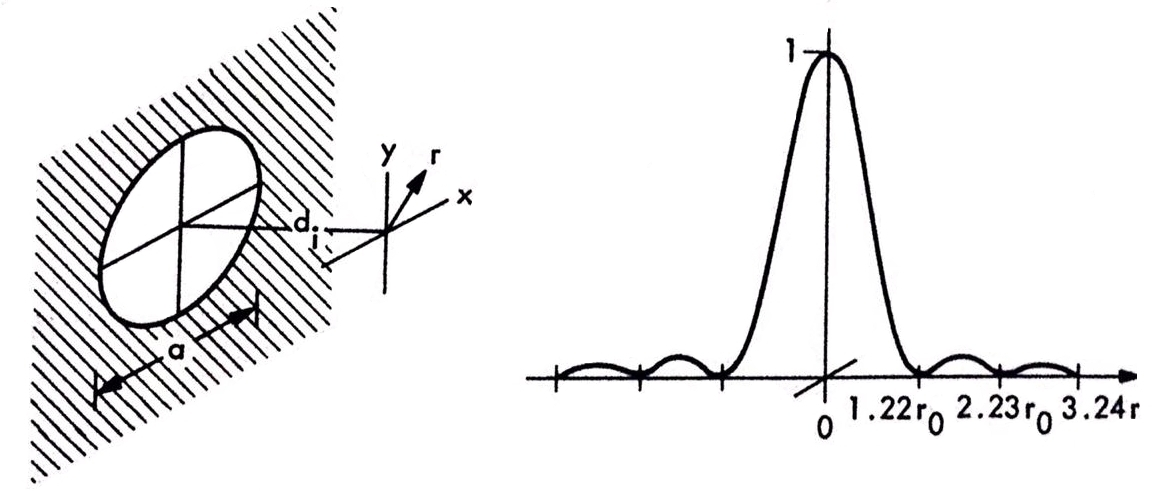
\includegraphics[scale=0.35]{images/discrete_psf_scheme.jpeg}
	\end{center}
	\centering
    \fadaptada{castleman1996digital}
\end{figure}

The discrete OTF is then the \sigla{DFT}{Discrete Fourier Transform} (explained in Chapter \ref{chapter:theoretical-background}) of the PSF in equation \ref{eqn:discrete_psf}. The OTF characterizes the intensities of light that emanate from the specimen in terms of frequencies. 

There is another property of image formation and acquisition that influences the image quality: the noise. Pursuant to \citeonline{wu2008microscope}, imaging is corrupted by intrinsic or extrinsic noise; the former is modelled by a Poisson distribution that influences each photon that reaches the sensor, and the latter is modelled by a Gaussian distribution that sums to the matrix of pixels. Details about noise are out of the scope of this work, since the degradation to be deeply explored is the defocus blur.

\section{Blur Characterization}


According to \citeonline{smith2007modern}, every optical system exhibits blur properties, in higher or lower proportions, due to the depth of focus and its adjustment. The defocus blur is caused by the incidence of light within an aperture with significant dimensions, where the source of light is not properly placed in accordance to the focal plane; it is related to the variables of the optical system such as depth of focus, aperture, depth of field, aberrations and so on \cite{joshi2014defocus}. Motion blur is caused by the attempt of taking pictures from moving objects and camera displacements; it can be caused in large scales (an image of a moving runner) or in small scales (live cell imaging). Both types of blur result in a loss of image details, sharpness and information. It can also be classified into global and partial blur. The former consists of a mathematically well-behaved homogeneous process and the latter is related to real world blurring phenomena. In light microscopy applications, the most relevant type is the partial defocus blur. Figure \ref{fig:defocus_motion_blur} shows an example of large scale defocus and motion blurs.

\begin{figure}[H]
	\centering
	\caption{\label{fig:defocus_motion_blur}Defocus blur (left) and motion blur (right) in large scales.}
	\begin{center}
	    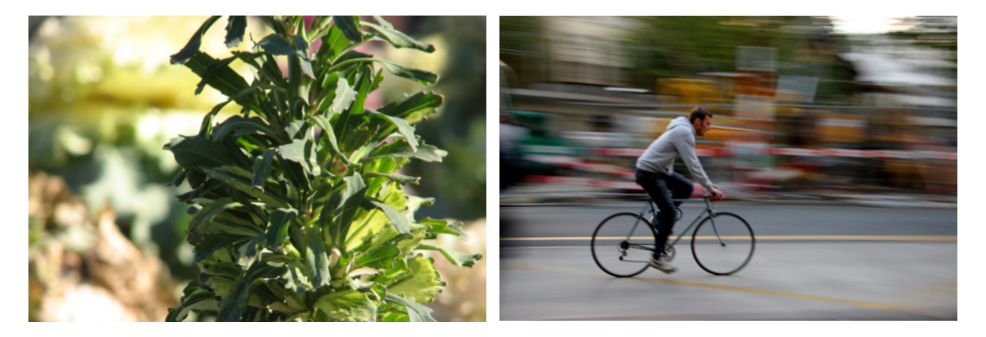
\includegraphics[scale=0.4]{images/fig7.png}
	\end{center}
	\centering
    \fadaptada{su2011blurred}
\end{figure}

\subsection{Point Spread Function}

Dirac delta functions are generalized functions designed for representing an impulse - a infinitely high value within a infinitely small period of time \cite{bracewell2000fourier}. In a nutshell, it is a function $\delta(x)$ that is zero-valued for any $x \neq 0$ and is infinity-valued for $x = 0$. This property can be combined with any smooth function $f\colon \mathbb{R}^{n} \to \mathbb{R}^{n}$, given  and provides the property shown in equation \ref{eqn:dirac_delta_function} in low dimension for didactic purposes. Figure \ref{fig:discrete_dirac_delta} illustrates the delta function on  $A = \{\, x\in \mathbb{R} \mid 0\le x\le 10^{7} \,\}$ normalized into the $[0,1]$ interval.

\begin{equation}
    \label{eqn:dirac_delta_function}
      \int^{\infty}_{-\infty}\delta(x-a)f(x) = f(a)
\end{equation}

\begin{figure}[H]
	\centering
	\caption{\label{fig:discrete_dirac_delta}Discrete representation of the Dirac delta function.}
	\begin{center}
	    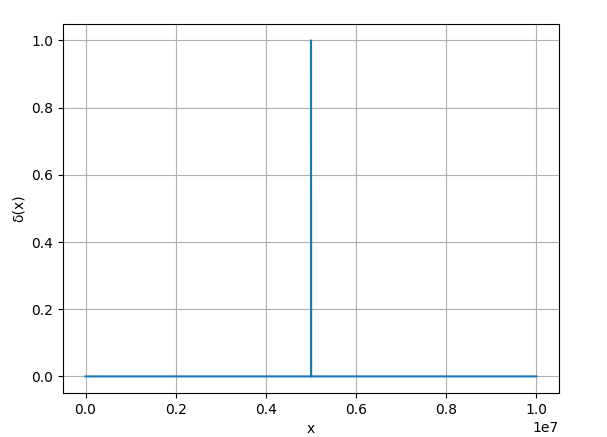
\includegraphics[scale=0.5, trim = {0 0.6cm 0 1.5cm}]{images/fig9.png}
	\end{center}
	\centering
    \fautor
\end{figure}

This concept of impulse is a light source with the shape of a point when it comes to images. It provides the effect of blurring on images, since it promotes the diffusion of the acquired information. Figure \ref{fig:psf} shows an arbitrary example of a punctual source of light and its image, which suffers the spreading effect.

\begin{figure}[H]
	\centering
	\caption{\label{fig:psf}Magnified image of a light impulse (left) and its impulse response function, the PSF (right).}
	\begin{center}
	    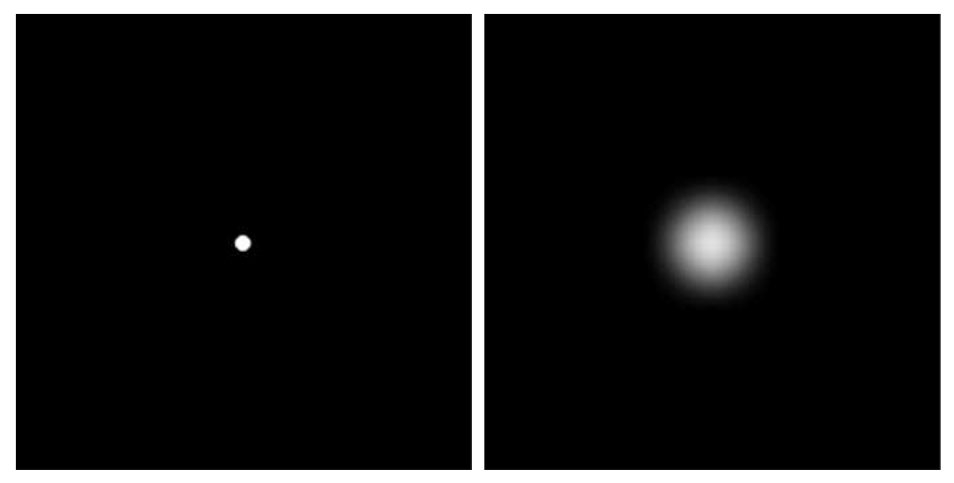
\includegraphics[scale=0.4]{images/fig8.png}
	\end{center}
	\centering
    \fadaptada{gonzalez2008digital}
\end{figure}

{\color{red}
Digital images can be considered as discrete representations of a continuous space, as the image acquisition consists in the action of several sensors that capture light from the environment and divide the information into pixels. Hence, the most trivial and used representation for digital images are matrices of pixels and can be described as functions that suffer the influence of other functions during acquisition. The degradation process which stands for the influence quoted before may be mathematically illustrated by equation \ref{eqn:degradation_model} \cite{gonzalez2008digital}:

\begin{equation}
    \label{eqn:degradation_model}
      g(x,y) = h(x,y) \ast f(x,y) + \eta(x,y)
\end{equation}

\noindent where $f(x,y)$ is the function that represents the original image from the scene, $g(x,y)$ is the degraded image, $\eta(x,y)$ is the additive noise function and $h(x,y)$ is the point spread function of the imaging system. The $\ast$ symbol represents the convolution operation: in conformity with \citeonline{bracewell2000fourier}, it is an integral that relates a function $f$ with a function $g$ by means of a weighted sum in the range of a variable $u$, and is denoted by equation \ref{eqn:convolution}:

\begin{equation}
    \label{eqn:convolution}
      \int^{\infty}_{-\infty}f(u)g(x - u)du
\end{equation}
}

Thus, the blurring process can be considered as a natural phenomenon guided by a convolution operation, but it may suffer interference of factors such as motion of the object, the scene or the camera and differences of the surface's topology when it comes to microscopy. 


{\color{red} TRANSFORMS AND FUSION SHOULD BE MOVED TO IMAGE PROCESSING CHAPTER}

% \section{Image Transforms}

% Usually, the most trivial image processing operations are done at the pixel level; they act on one of the channels of an image from an specific color space, on gray levels of a grayscale image and so on. Some procedures such as the convolution have the computational performance as a bottleneck, and this is one of the reasons why \emph{image transforms} are widely used. They encompass any group of mathematical operations that takes the input signal or the input image out of their domain an project them onto the transformed domain \cite{gonzalez2008digital}. The convolution operation, for instance, turns itself into a simple matrix multiplication task on the Fourier Transform domain (which will be detailed in the following sections) and that solves the performance bottleneck. The general structure of a forward image transform and an inverse image transform is denoted by  the pair of equations \ref{eqn:generic_transform}, respectively:


% \begin{align}
%     \label{eqn:generic_transform}
%     T(u,v) = 
%     \sum_{x=0}^{M-1}
%     \sum_{y=0}^{N-1}f(x,y)r(x,y,u,v)
%     &&
%     f(x,y) = 
%     \sum_{x=0}^{M-1}
%     \sum_{y=0}^{N-1}T(u,v)s(x,y,u,v)
% \end{align}

% \noindent where $M$ and $N$ are the dimensions of the image, $x$ and $y$ are coordinates of the image, $u = \{0,1,2,...,M-1\}$ and $v = \{0,1,2,...,N-1\}$ are called transform variables, $r(x,y,u,v)$ is a function named \emph{forward transform kernel} that is responsible for the forward domain change and finally $s(x,y,u,v)$ is the inverse kernel for $r$. These equations take an image to another domain, perform some operations and then return to the spatial domain. These are the common steps in transforms applications indeed. The following sections contain details about relevant image transforms in image segmentation and image fusion.

% \subsection{Fourier Transform}

% The Fourier Transform is a mathematical framework that expresses a periodic or non-periodic function with a sum of weighted sinusoids, what results in a set of different frequencies \cite{gonzalez2008digital}. The transform relies on complex numbers and the Euler's formula. The complex numbers belong to the broadest of the number sets, i.e. $\mathbb{R} \subseteq \mathbb{C}$, and consists of a \emph{real part} $a$ and an \emph{imaginary part} $bj$, shown by equation \ref{eqn:complex_number}:

% \begin{equation}
% \label{eqn:complex_number}
%     z = a + bj
% \end{equation}

% \noindent where $j = \sqrt{-1}$ is the imaginary unit. In this sense, the Euler's formula relates complex exponential functions with trigonometric functions through the equation  \ref{eqn:euler_formula}:

% \begin{equation}
% \label{eqn:euler_formula}
%     e^{j\theta} = \cos{\theta} + j\sin{\theta}
% \end{equation}

% \noindent where $\theta \in \mathbb{R}$ is a number that represents an angle in radians. This is the fundamental framework to describe the Fourier transform, since it is a sum of function representations by means of the Euler's formula. According to \citeonline{brigham1988fast}, the Continuous and the \sigla{DFT}{Discrete Fourier Transform} in a simplified version can be computed as shown on the left and on the right of Equation \ref{eqn:fourier_transform}, respectively:

% \begin{align}
% \label{eqn:fourier_transform}
%     H(x) = \int_{-\infty}^{\infty}h(t)e^{-j2 \pi tx}dt
%     &&
%     H(x) = \sum_{x=0}^{N-1}h(t)e^{-j2 \pi t \frac{x}{N}}
% \end{align}

% \noindent with $H(x)$ as the Fourier transform of a function $h(t)$, $t$ represents functions is the time domain, $x$ represents the frequency domain and $N$ represents the total number of samples on the discrete approach. As already pointed out, images can be interpreted as two-dimensional functions; hence, the most important version of the Fourier transform in the context of image processing is the two-dimensional DFT, given by Equation \ref{eqn:2D_dft}:

% \begin{equation}
% \label{eqn:2D_dft}
%     H(u,v) = \frac{1}{\sqrt{MN}}\sum_{x=0}^{M-1}\sum_{y=0}^{N-1}h(x,y)e^{-j2 \pi \big(\frac{ux}{M} + \frac{vy}{N}\big)}
% \end{equation}

% \noindent where $h(x,y)$ consists of an image, $M$ and $N$ are the image dimensions and $u$ and $v$ are coordinates in the frequency domain. This operation is extremely useful for almost every field related to analysis of functions. However, the DFT consists of a convolution process with $O(n^{2})$ asymptotic complexity, which can be too slow for larger dimensions. The \sigla{FFT}{Fast Fourier Transform} is an algorithm to compute the DFT by taking small slices of the signal, computing the transform with them and them merging the result. This procedure is performed in $O(n \log n)$ complexity, which is reasonable for many applications.


% \section{Image Fusion}

% Immediately upon the blur map extraction is satisfactorily complete, an image fusion operation is needed in order to achieve the highest amount of focused regions as possible. Image fusion is a process that merges several images (possibly taken in diverse conditions or with different cameras) into one image with higher quality, more details and consequently more useful for humans and computer tasks \cite{mitchell2010image}. Image fusion techniques can be used in noise reduction, edge enhancement and super-resolution, for example. 

% One prominent use of image fusion occurs in medical image fields; the quality of information about illnesses, cells, clinical analysis and several other medical tasks (including the computer assisted ones) have found profitable results from the techniques and lead themselves to better and faster decisions when it comes to human beings \cite{james2014medical}.

% There are relevant applications in remote sensing multispectral images, segmentation of regions in different colourspaces, biometry: the pan-sharpening process is the generation of an high resolution multispectral image from low to high resolution ones, K-Means segmentation and fusion of pixels in the \sigla{RGB}{Red, Green and Blue colourspace} and the Iris Recognition biometric process with video frames are examples of such tasks, respectively \cite{mitchell2010image}.

% \subsection{General Framework}

% Still according to \citeonline{mitchell2010image}, the general framework for the image fusion procedure can be accomplished in four stages: Multiple Input Images, Common Representational Format, Fusion and Display.
% The \emph{multiple input images} stage consists in obtaining the set of images which will be merged. There are several approaches to this: the dataset may be captured from different sensors, on distinct light conditions or angles, with different magnifications, on several focus and with temporal measurements if the scene changes through time.

% After the image set generation, there is the necessity of reshaping each item. This configures the \emph{common representational format}, responsible for creating a new and temporary dataset with the same properties, e.g. colourspace, dimensions, noise level and so on. The \emph{fusion} stage consists of using a decision method in order to dictate which regions, objects, colours or details will compose the final image; this can be done by any approach that relates to how the result should be. There are some methods that rely on the Wavelet Transform domain, for example. Finally, the \emph{display} stage consists in providing a view for the resulting image, which can be used directly for any further task or even be the input for other image processing operation. Figure \ref{fig:fusion_general_framework} depicts an arbitrary example of the four stages:

% \begin{figure}[H]
% 	\centering
% 	\caption{\label{fig:fusion_general_framework}Image fusion general framework. (a) Multiple Input Images, (b) Common Representational Format, (c) Fusion and (d) Display.}
% 	\begin{center}
% a 	    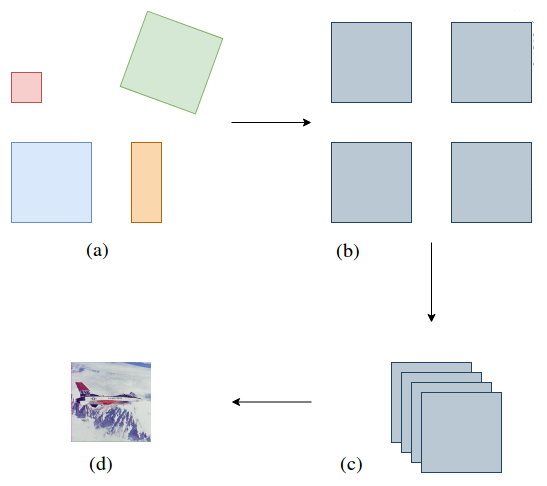
\includegraphics[scale=0.4]{images/fig10.png}
% 	\end{center}
% 	\centering
%     \fautor
% \end{figure}

% The four arbitrary images in Figure \ref{fig:fusion_general_framework}.\textbf{(a)} represents different images of the same scene, taken at different resolutions, rotations and shapes. In \ref{fig:fusion_general_framework}.\textbf{(b)}, the images are all reshaped, converted to the same colourspace and ready to receive processing algorithm which will transform them into feature vectors. Figure \ref{fig:fusion_general_framework}.\textbf{(c)} represents the image fusion by means of an arbitrary method. The resulting image is depicted in Figure \ref{fig:fusion_general_framework}.\textbf{(d)}.

% Since image fusion is only one branch of data fusion field, this procedure has a wide variety approaches and methods; hence, the domain will be restricted to the multifocus image fusion and some related work will be presented as follows, in section \ref{sec:multifocus_image_fusion}.
